Im folgenden Bild ist noch einmal das Gantt-Chart dargestellt, das zu Beginn der Implementierungsphase erstellt wurde.

\begin{figure}[H]
	\centering
	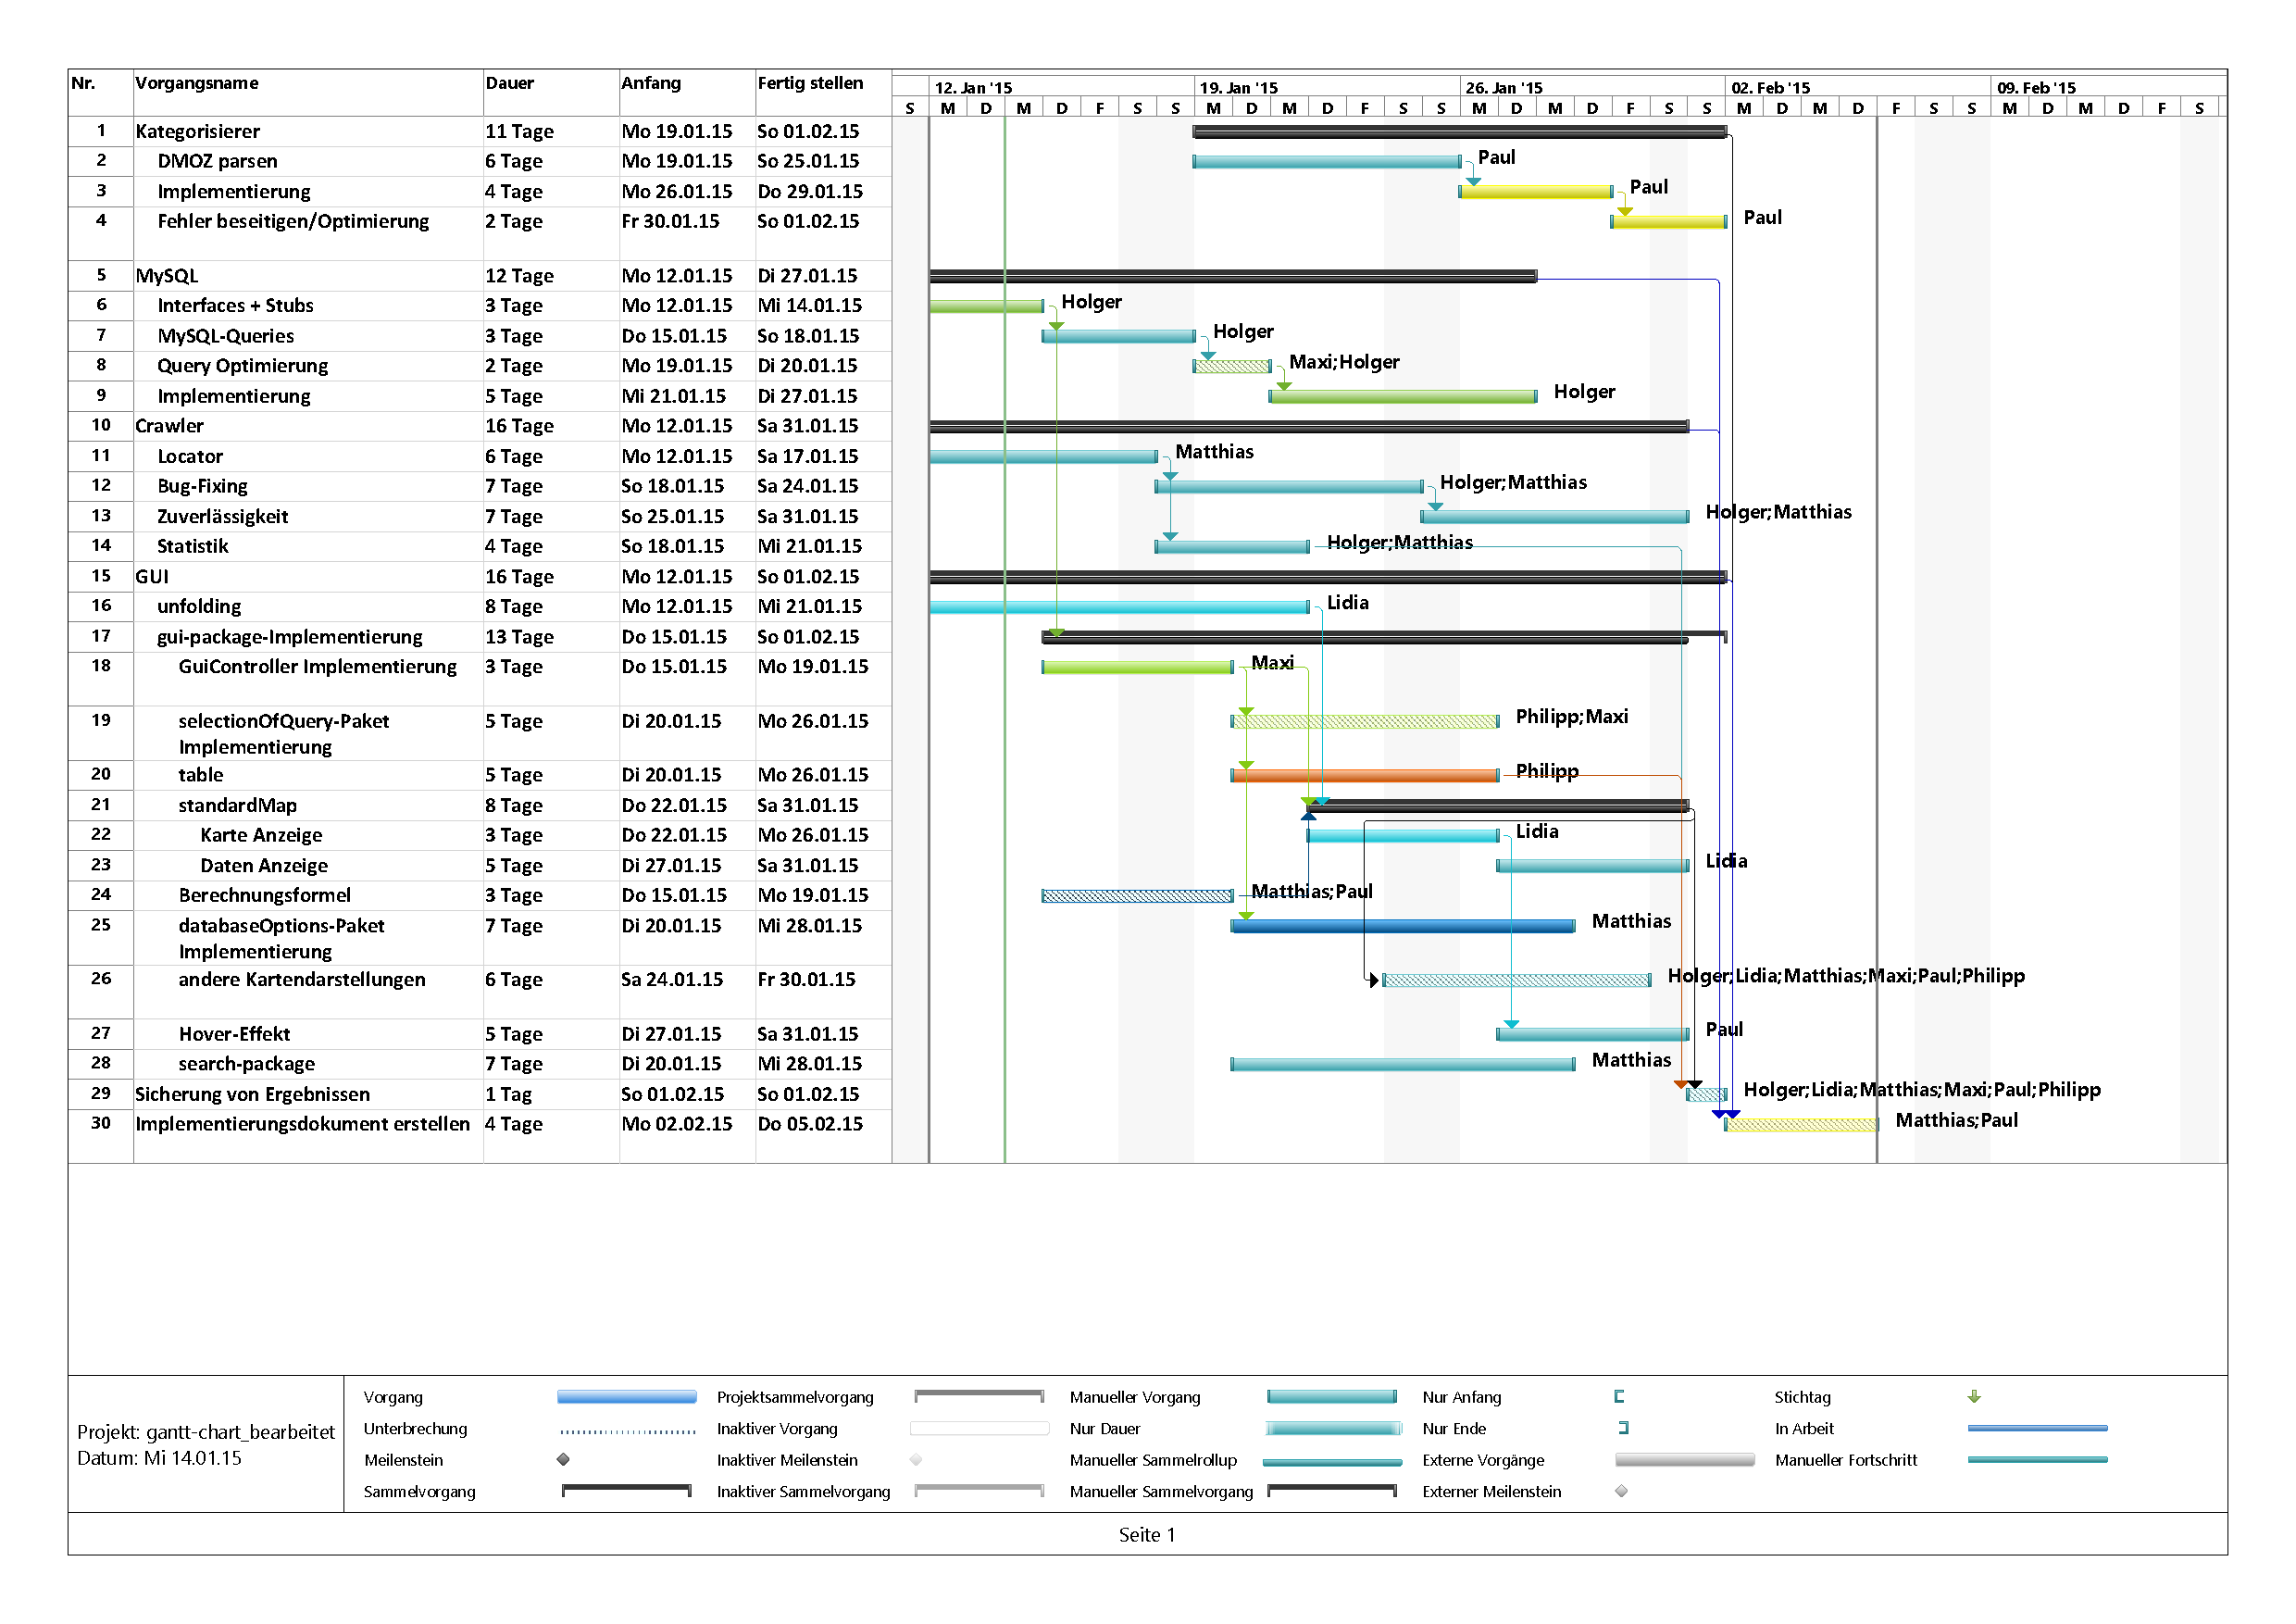
\includegraphics[width=\textwidth]{../Gantt/Implementierungsplan.pdf}
	\caption{Der zu Beginn der Implementierungsphase erstellte Implementierungsplan}
\end{figure}

Im Laufe der Implementierung wurde anhand dieses Dokuments regelmäßig der Status des Projekts beurteilt und der Fortschritt festgestellt. Dabei musste in den folgenden Fällen vom Plan abgewichen werden:
\begin{itemize}
	\item Das Parsen der DMOZ-Datenbank und das Implementieren einer ersten Version des Kategorisierers verlief deutlich schneller als geplant. Dies war bereits zu Beginn der Woche vom 26.1. erledigt. Leider ließen sich jedoch nicht einmal 3000 der 90000 Accounts anhand einer URL-Übereinstimmung kategorisieren. Die Aufgabe "`Fehler beseitigen/Optimierung"' nahm daher etwas mehr Zeit in Anspruch, sodass jetzt immerhin fast 6000 Accounts kategorisiert werden konnten.
	\item Im Bereich MySQL wurde der vorgesehene Zeitrahmen einhalten. Jedoch wurde die Phase "``Query Optimierung"' in beide Richtungen auch über die anderen Aufgaben hin erweitert. Neben der Steigerung der Effizienz durch Indizes über bestimmten Spalten wurde auch versucht, die jeweiligen MySQL-Nutzer mit einer minimalen Menge an Rechten auskommen zu lassen.
	\item Die Implementierung des Crawlers größtenteils wie im Gantt-Chart geplant. Da immer wieder Fragen einer Verbessrung des Webdienstes auftraten, verzögerte sich die Implementierung des Locators um wenige Tage.
	\item Im Bereich der Kartendarstellungen gab es dagegen größere Abweichungen vom Plan. Die verwendete Bibliothek "`unfolding"' erwies sich als nicht kompatibel mit JavaFX. So wurde zunächst versucht die Karte über einen sog. SwingNode in JavaFX einzubinden. Nachdem auch das fehlschlug, wurde die Karte als externes Swing-Fenster implementiert. Die hiervon abhängenden Punkte sind somit jeweils um mehrere Tage nach hinten verschoben worden. Das optionale "`search"'-Package konnte dann leider nicht mehr implementiert werden.
	\item Die Implementierung der Berechnungsformel benötigte sechs der bedachten drei Tage, da noch nicht genau feststand, in welchem die entsprechenden Daten wo liegen.
	\item Die eigentliche Implementierung des "`GUIController"' verlief im Zeitplan. Jedoch wurden nachträglich aufgrund von Änderungen anderer Pakete immer wieder noch einzelne Methoden hinzugefügt werden. So zum Beispiel Methoden zum Anzeigen der Detailinformationen.
\end{itemize}

Folgend eine aktualisierte Version des Gantt-Charts.

\begin{figure}[H]
	\centering
	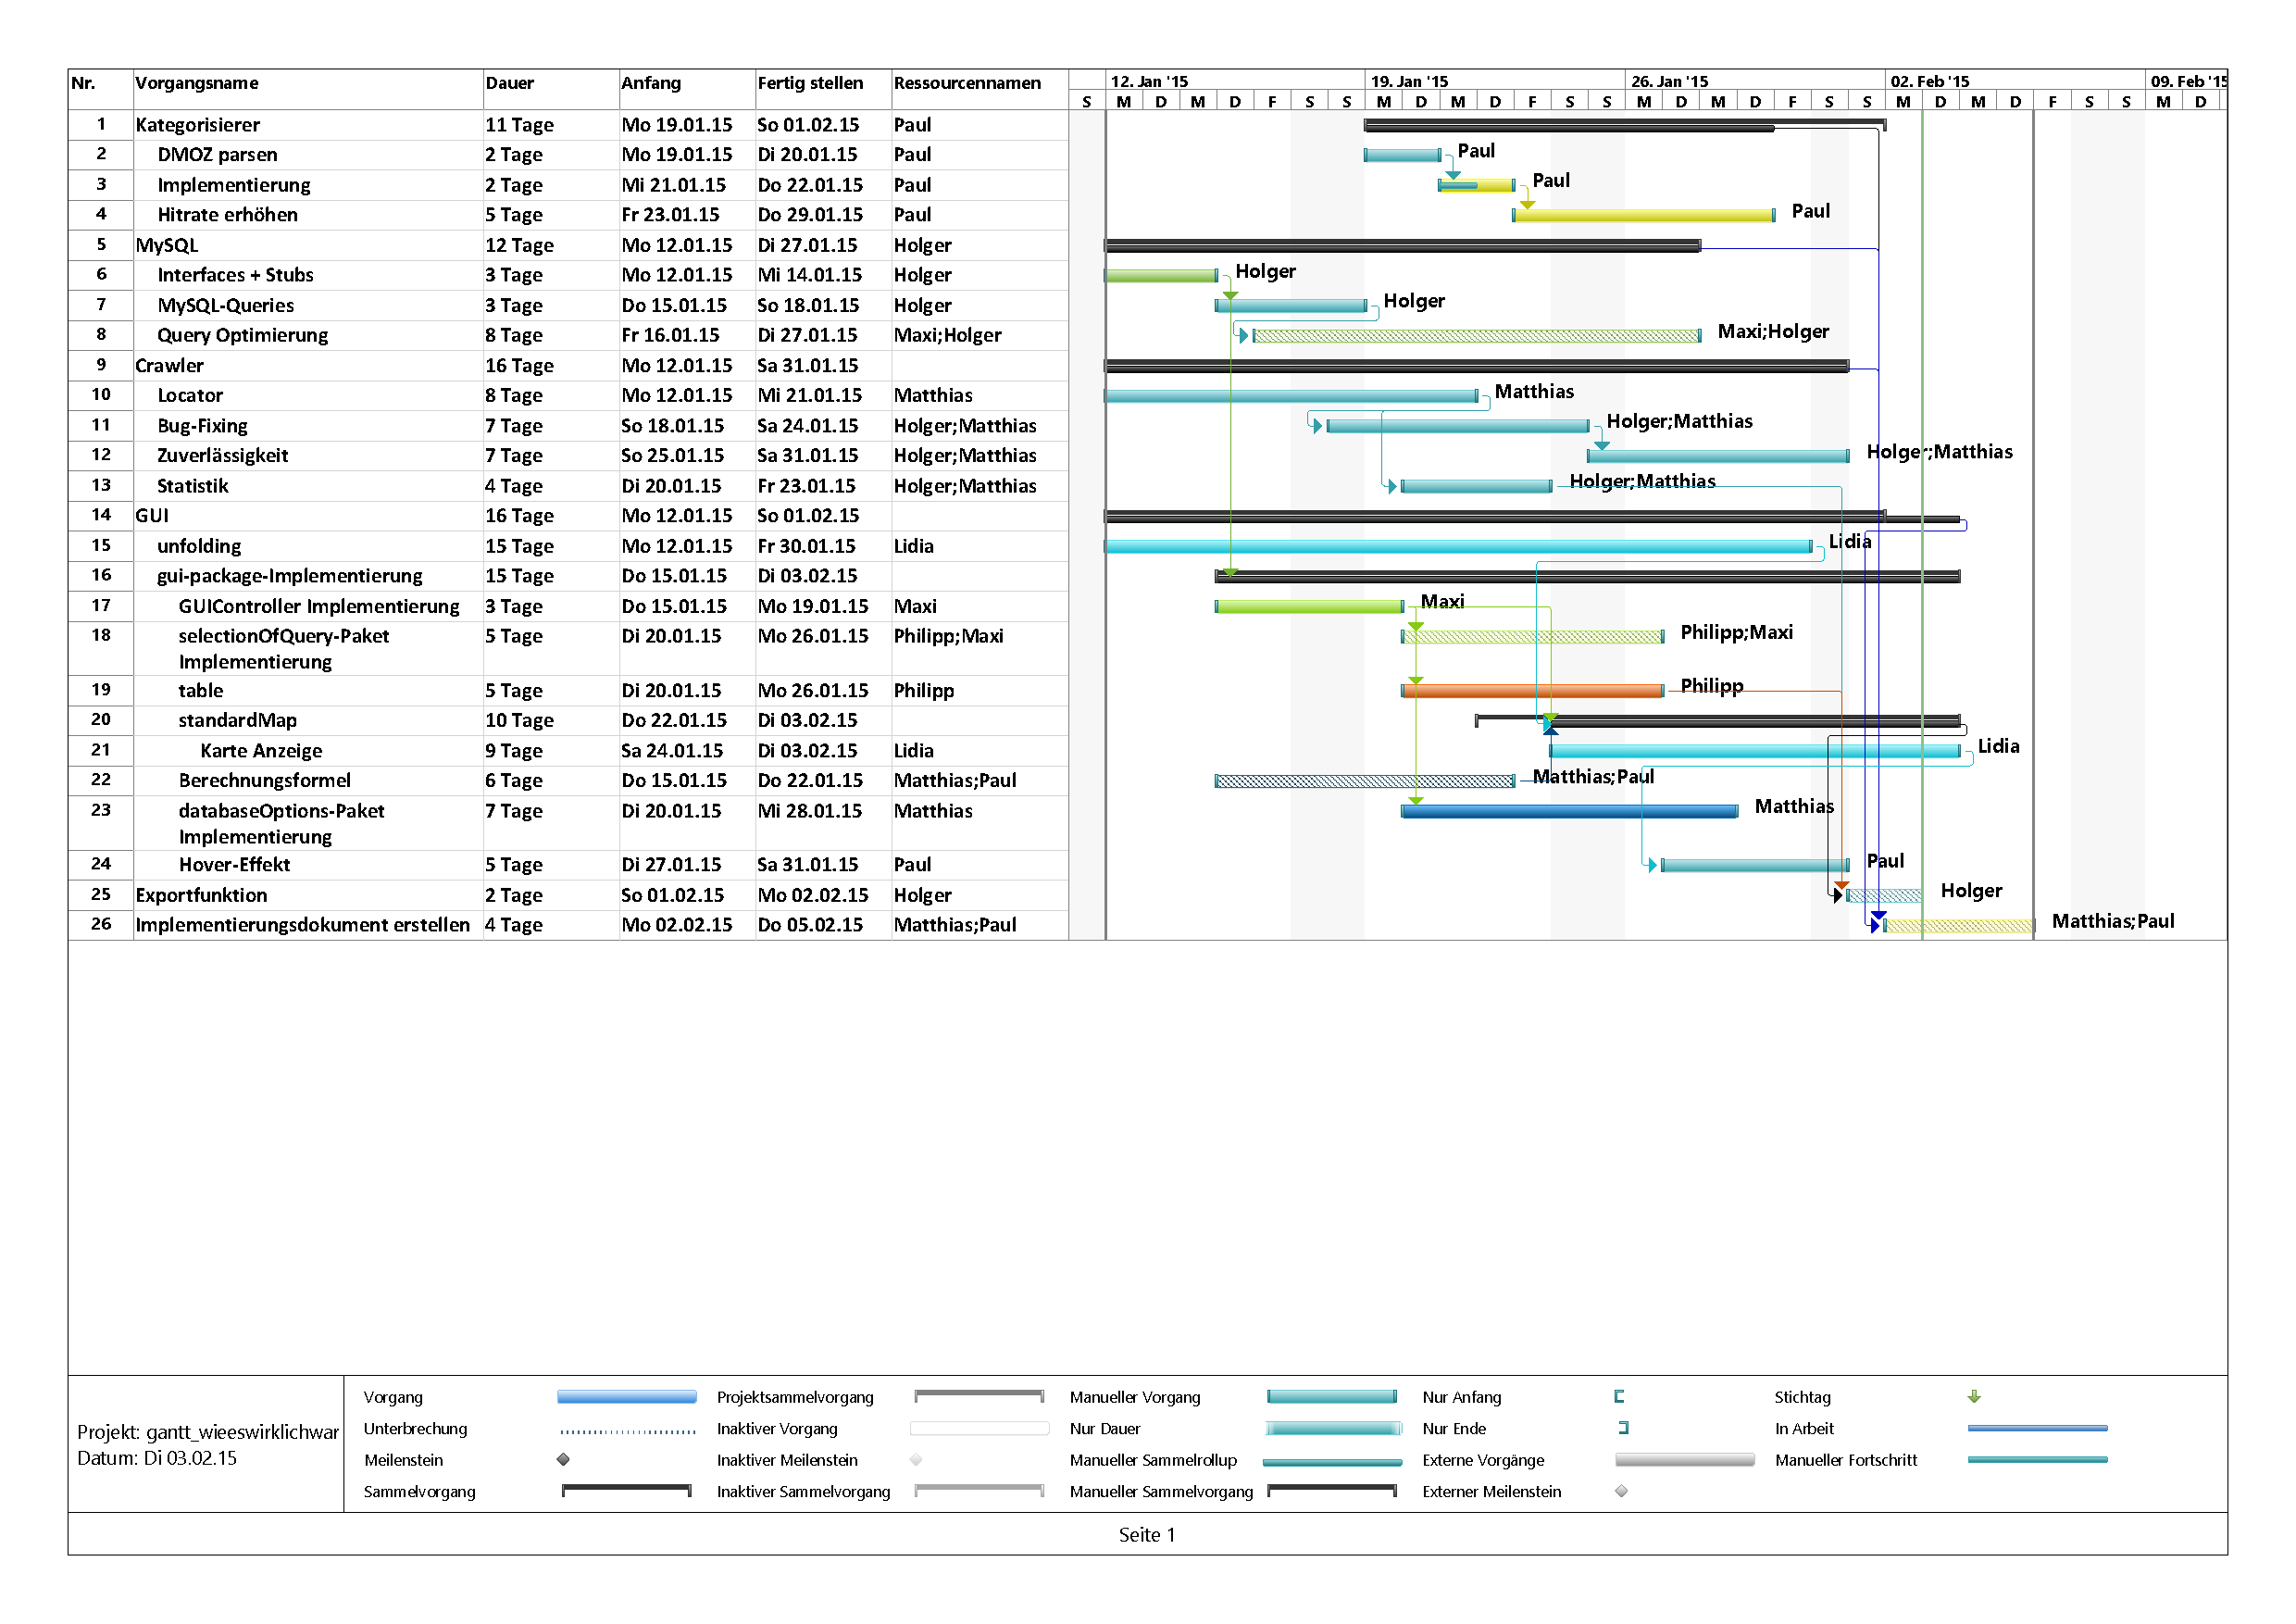
\includegraphics[width=\textwidth]{../Gantt/gantt_neu.pdf}
	\caption{Rückblickend erstelltes Gantt-Chart}
\end{figure}
